A landing page was created to give the entire application a more complete look, and instead of dropping the user directly into the application some information about the developers, the application, the technologies and a visual demonstration in the form of a GIF that shows how a basic workflow with Seatgen could look like. The landing page also has a similar color scheme to the actual application, but it is way more visually pleasing and filled with more animations and gradients, because SeatGen focuses more on the functionality and the speed of the workflow instead of fancy animations that could just distract the user from the work. The landing page is shown in figure \ref{fig:landing-page}.

\begin{figure}[H]
    \centering
    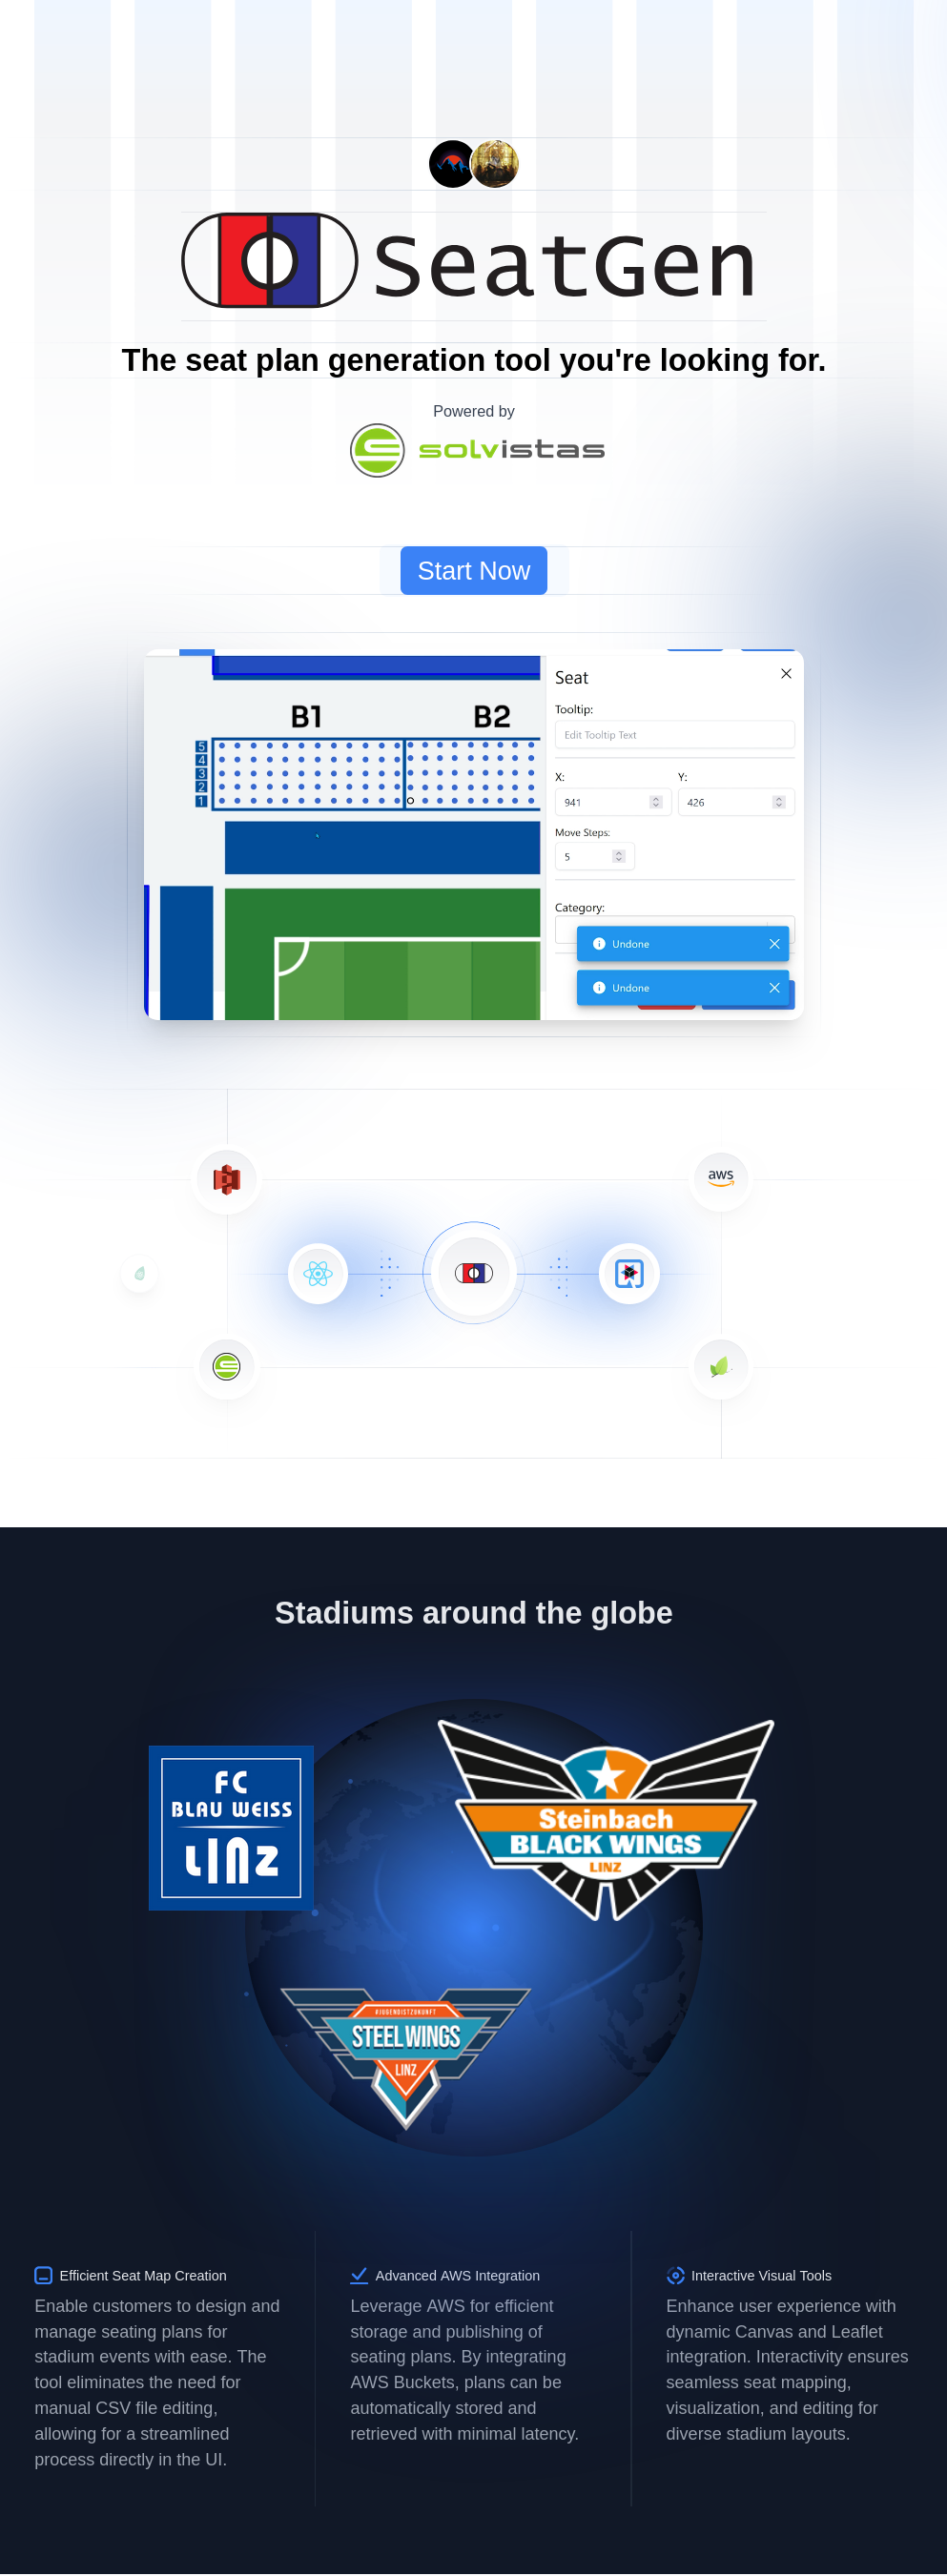
\includegraphics[scale=0.3]{pics/landing-page.png}
    \caption{Landing Page}
    \label{fig:landing-page}
\end{figure}
\newpage